\clearpage
\chapter{Vorgehensweise}
\section{Task-Technology-Fit Theorie}

\improvement{Einstieg Bennardo anschauen}

Das Ziel dieser Projektarbeit ist es, die Eignung der SAP BTP als digitale Plattform für Kfz-Versicherer zu untersuchen. Hierfür sollen zunächst die Anforderungen der Kfz-Versicherer an technische Plattformen identifiziert und anschließend mit den Funktionen und Services der SAP Business Technology Platform verglichen werden.

Zur Unterstützung dieser Analyse wird das Task-Technology-Fit (TTF) Modell (TTF) von Goodhue und Thompson verwendet, welches in Abblidung \ref{fig:TTF} dargestellt ist. Es vergleicht die Charakteristiken einer bestimmten Aufgabe mit den Charakteristiken einer bestimmten Technologie, die zur Erfüllung dieser Aufgabe verwendet werden soll. Gemäß Goodhue et. al (1995) kann eine Technologie nur dann eine positive Auswirkung auf die Leistung von Einzelpersonen oder Organisationen haben, wenn eine Übereinstimmung zwischen den Funktionalitäten der Technologie und den Anforderungen der Nutzer besteht. Die Leistungen werden umso positiver beeinflusst, je besser die Technologie mit der zu unterstützenden Aufgabe übereinstimmt.\autocite[Vgl.][S. 214-216]{GOODHUE1995}


%\autocite[Vgl.][S. 215]{GOODHUE1995}
%\autocite[Vgl.][S. 399]{SPIES2020}

\begin{figure}[h]
    \centering
    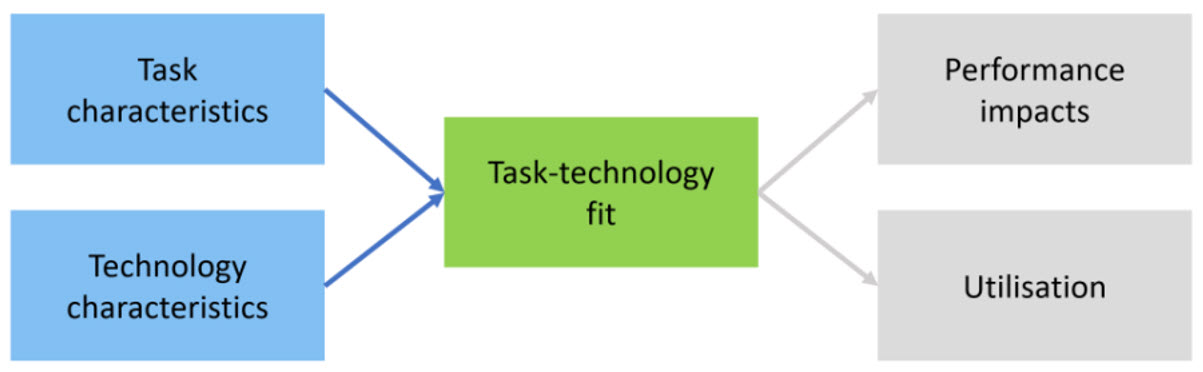
\includegraphics[width=0.9\textwidth]{img/TTF_Nadine.jpg}
    \caption[Modell der Task-Technology-Fit Theorie]{Modell der Task-Technology-Fit Theorie\autocite{TTF}}
    \label{fig:TTF}
\end{figure}
\footnotetext{Vgl. eigene Darstellung angelehnt an: Goodhue und Thompson, 1995, S. 215.}
\improvement{Frage ob man in der Grafik utilization darstellt, da es sowohl für meine Arbeit als auch für den Text nicht relevant ist}

Das TTF-Modell kann auf jeder Abstraktionsebene angewendet werden, da die aus der Anforderungsübereinstimmung resultierenden Produktivitätsverbesserungen nicht auf einzelne Personen beschränkt sind und auch für ganze Teams oder komplette Organisationen auftreten können.\autocite[Vgl.][S. 1827f]{GOODHUE1995b} 


%Hierbei kann die TTF-Analyse auf verschiedenen Abstraktionsebenen durchgeführt werden, da die Vorteile der Verbesserung der Produktivität nicht nur auf Einzelpersonen, sondern auch auf ganze Organisationen übertragen werden können.\autocite[Vgl.][S. 1827f]{GOODHUE1995b} Eine verbesserte Leistung kann gemäß TTF auf die reibungslose Ausführung der Aufgabe, die Verringerung der Kosten für die Ausführung der Aufgabe oder die Erleichterung der Aufgabe zurückzuführen. \autocite[Vgl.][S. 96]{LEE2007}

Die Task Charakteristiken beziehen sich dabei auf die Gesamtheit der physischen und kognitiven Handlungen und Prozesse, welche von einer Organisation oder einer Einzelperson in einer bestimmten Umgebung ausgeführt werden. Sie werden speziell in Bezug zur Technologie, welche sie bei der Ausführung unterstützen soll, betrachtet und je nach Komplexität auf unterschiedliche Detailebenen heruntergebrochen. \autocite[Vgl.][S. 398]{SPIES2020} Nach Goodhue (1998) können die zur Evaluation der Technologie notwendigen Anforderungen mithilfe eines Task-Modells, einer Literaturrecherche oder mittels Interviews erhoben werden.\autocite[Vgl.][S. 126]{GOODHUE1998} Eine Anforderung wird in diesem Kontext definiert als eine Aussage, \enquote{die einen Bedarf und die damit verbundenen Einschränkungen und Bedingungen darstellt und erläutert}.\autocite[Vgl.][]{ISO2017}

Innerhalb des TTF-Modells beziehen sich die Technologie Charakteristiken auf die Werkzeuge, welche von Einzelpersonen zur Ausführung ihrer Aufgaben verwendet werden oder diese bei der Ausführung ihrer Aufgaben unterstützen.\autocite[Vgl.][S. 399]{SPIES2020} Dabei kann sowohl der Einfluss eines einzelnen Systems, als auch die Wirkung einer Gesamtheit von bereitgestellten Systemen und Diensten betrachtet werden. \autocite[Vgl.][S. 216]{GOODHUE1995}

%Als Technologie Charakteristiken werden im Rahmen des TTF Modells die Werkzeuge bezeichnet, welche von Einzelpersonen zur Ausführung ihrer Aufgaben oder zur Unterstützung bei der Ausführung ihrer Aufgaben verwendet werden sollen.\autocite[Vgl.][S. 216]{GOODHUE1995} Dabei ist das Modell so allgemein gehalten, dass es sich entweder auf die Einfluss eines bestimmten Systems oder auf die umfassendere Wirkung der Gesamtheit der bereitgestellten Systeme, Strategien und Dienste ausgerichtet sein kann. \autocite[Vgl.][S. 399]{SPIES2020}








\newpage
\section{Systematische Literaturanalyse}


Im Rahmen des Task-Technology-Fit Models wurde eine systematische Literaturanalyse zur Identifikation der Anforderungen der Kfz-Versicherer an digitale Plattformen durchgeführt. Hierfür wurden zunächst die für die Task Charakteristika relevante Suchbegriffe auf Deutsch und Englisch festgelegt., siehe Tabelle … im Anhang. Daraufhin wurde mithilfe dieser Suchbegriffe die Datenbanken Google Scholar, EBSCO Discovery Service (aufgerufen über die Metasuche der DHBW Mannheim), JSTOR sowie WISO nach Fachliteratur, internationale und nationale Zeitschriften, Studien, Magazinen und Internetartikeln  durchsucht. Die dabei angewendeten Suchkriterien sind in Tabelle .. im Anhang aufgezeigt.  Grundlage für die Betrachtung der Recherche-Ergebnisse waren der Abstract, die Gliederung, die Einleitung sowie das Fazit. Dabei wurden die ausgewählte Literatur zur Identifikation der Task Charakteristika als Ganzes oder in Ausschnitten gelesen und analysiert. Vgl (Sribbr)


\newpage
\section{Semistrukturiertes Leitfadeninterview und qualitative Inhaltsanalyse}
\newpage